\documentclass[10pt,border=5pt]{standalone}
\usepackage[T1]{fontenc}
\usepackage{lmodern,amsmath,amssymb,mathrsfs,tikz}
\usetikzlibrary{arrows.meta,positioning,calc}
\definecolor{ink}{HTML}{192536}
\definecolor{blue}{HTML}{2E70AE}
\definecolor{gold}{HTML}{A66A15}
\definecolor{green}{HTML}{28764D}
\definecolor{red}{HTML}{B43D3D}
\newcommand{\C}{\mathbb C}
\newcommand{\R}{\mathcal R}
\newcommand{\Lr}{\mathcal L_{\mathrm{res}}}
\newcommand{\Prs}{\mathcal P_{\mathrm{res}}}
\newcommand{\Tr}{T_{\mathrm{resp}}}
\newcommand{\rr}{\rho_{\mathrm{res}}}
\tikzset{every node/.style={font=\small,text=ink,align=center},
 box/.style={draw=blue,fill=blue!4,rounded corners=3pt,line width=.7pt,inner sep=7pt},
 goldbox/.style={box,draw=gold,fill=gold!5},
 greenbox/.style={box,draw=green,fill=green!5},
 redbox/.style={box,draw=red,fill=red!4},
 edge/.style={-{Stealth[length=4pt]},draw=ink,line width=.7pt},
 heading/.style={font=\small\bfseries},
 note/.style={font=\small,text=ink!85}}

\begin{document}
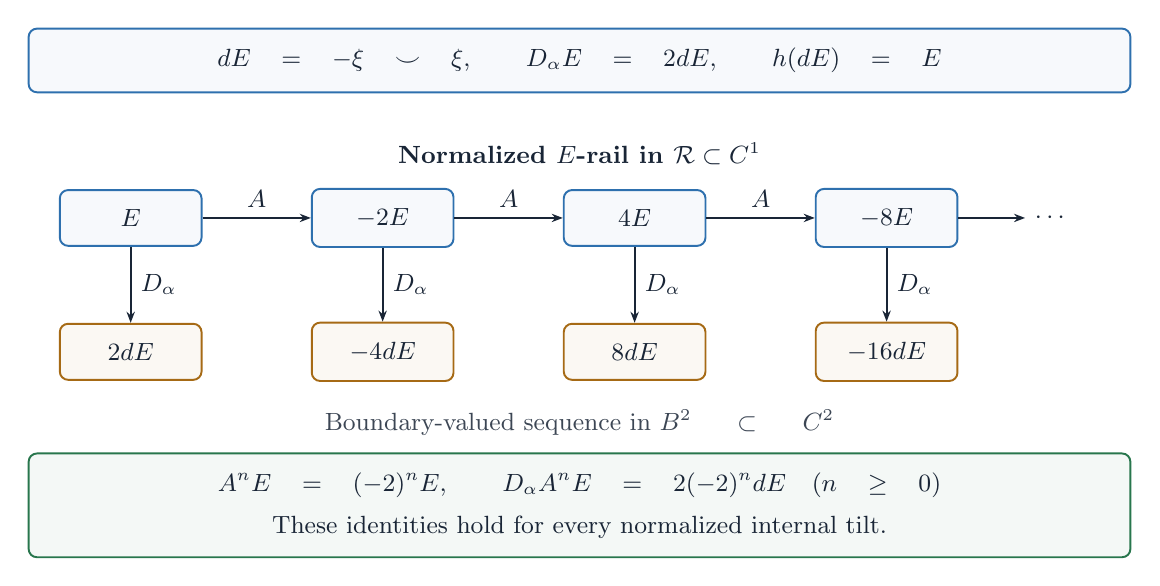
\begin{tikzpicture}
\node[box,text width=13.5cm] (ident)
 {$dE=-\xi\smile\xi,\qquad D_\alpha E=2dE,\qquad h(dE)=E$};
\node[heading,below=5mm of ident] (title) {Normalized $E$-rail in $\R\subset C^1$};
\node[box,minimum width=18mm] (e0) at (-5.7,-2) {$E$};
\node[box,minimum width=18mm] (e1) at (-2.5,-2) {$-2E$};
\node[box,minimum width=18mm] (e2) at (.7,-2) {$4E$};
\node[box,minimum width=18mm] (e3) at (3.9,-2) {$-8E$};
\node (etc) at (6,-2) {$\cdots$};
\draw[edge] (e0)--node[above]{$A$}(e1);
\draw[edge] (e1)--node[above]{$A$}(e2);
\draw[edge] (e2)--node[above]{$A$}(e3);
\draw[edge] (e3)--(etc);
\node[goldbox,minimum width=18mm] (b0) at (-5.7,-3.7) {$2dE$};
\node[goldbox,minimum width=18mm] (b1) at (-2.5,-3.7) {$-4dE$};
\node[goldbox,minimum width=18mm] (b2) at (.7,-3.7) {$8dE$};
\node[goldbox,minimum width=18mm] (b3) at (3.9,-3.7) {$-16dE$};
\draw[edge] (e0)--node[right]{$D_\alpha$}(b0);
\draw[edge] (e1)--node[right]{$D_\alpha$}(b1);
\draw[edge] (e2)--node[right]{$D_\alpha$}(b2);
\draw[edge] (e3)--node[right]{$D_\alpha$}(b3);
\node[note,text width=13.5cm] at (0,-4.6)
 {Boundary-valued sequence in $B^2\subset C^2$};
\node[greenbox,text width=13.5cm] at (0,-5.65)
 {$A^nE=(-2)^nE,\qquad D_\alpha A^nE=2(-2)^n dE\quad(n\geq0)$\\[4pt]
 These identities hold for every normalized internal tilt.};
\end{tikzpicture}
\end{document}
